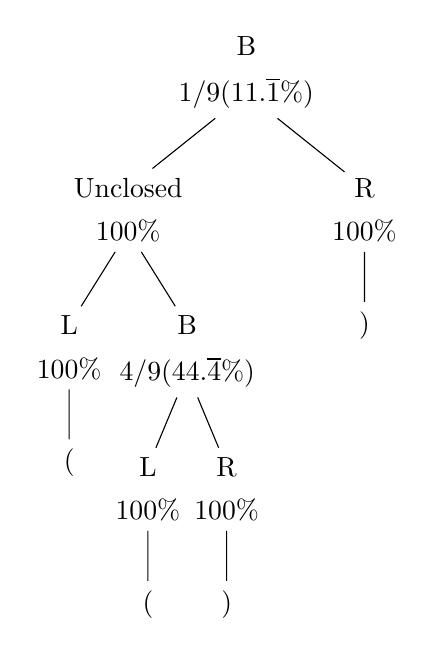
\begin{tikzpicture}[
    level distance=12mm,
    level/.style={sibling distance=30mm/#1}
]
  \node {B}
    % This node is placed at the very start of the children's paths
    node[below=8pt] {$1/9 (11.\overline{1}\%)$}
    child {node {Unclosed}
       node[below=8pt] {{$100\%$} }
      child {node {L} node[below=8pt] {{$100\%$} } child {node {(}}}
      child {node {B}
        node[below=8pt] {{$4/9 (44.\overline{4}\%)$} }
        child {node {L} node[below=8pt] {{$100\%$} } child {node {(}}}
        child {node {R} node[below=8pt] {{$100\%$} } child {node {)}}}
      }
    }
    child {node {R} node[below=8pt] {{$100\%$} } child {node {)}}};
\end{tikzpicture}